\documentclass[letterpaper, 10 pt, conference]{ieeeconf}
\usepackage[utf8]{inputenc}
\usepackage[ruled,algosection,vlined]{algorithm2e}
\usepackage{tikz}

\let\proof\relax
\let\endproof\relax
\usepackage{mathtools}
\usepackage{amsmath}
\usepackage{amsfonts}
\usepackage{amsthm}
\usepackage{amssymb}
\usepackage{mathrsfs}


\let\labelindent\relax
\usepackage{enumitem}

\usetikzlibrary{arrows,decorations,positioning,fit}

\IEEEoverridecommandlockouts
\overrideIEEEmargins
%\pdfobjcompresslevel=0
%\pdfminorversion=4

% See the \addtolength command later in the file to balance the column lengths
% on the last page of the document

\bibliographystyle{./IEEEtran}

\title{\LARGE \bf
On Detection of Influential Users and Content on Reddit*
}


\author{Rollen S. D'Souza$^{1}$%
  \thanks{*This work was not supported by any organization}%
  \thanks{$^{1}$Rollen S. D'Souza is a graduate student in the
    Department of Electrical and Computer Engineering,
    Faculty of Engineering,
    University of Waterloo,
    \texttt{rollen.dsouza@uwaterloo.ca}
  }%
}

% STYLING
\theoremstyle{definition}
\newtheorem{assumption}{Assumption}[section]
\newtheorem{claim}{Claim}[section]
\newtheorem{definition}{Definition}[section]
\newtheorem{theorem}{Theorem}[section]

% DEFINITIONS
\let\ker\relax
\DeclareMathOperator{\rank}{rank}
\DeclareMathOperator{\ker}{ker}
\newcommand{\R}{\mathbb{R}}

\tikzset{%
  post/.style={rectangle,draw=blue!70,top color=white,bottom color=blue!20,very thick},
  user/.style={circle,top color=white,draw=red!70,bottom color=red!20,very thick},
  plain/.style={rectangle,draw=black!70,top color=white, bottom color=black!20,very thick}%
}
%

\newcommand{\red}{\color{red}}

\begin{document}
\maketitle
\thispagestyle{empty}
\pagestyle{empty}


%%%%%%%%%%%%%%%%%%%%%%%%%%%%%%%%%%%%%%%%%%%%%%%%%%%%%%%%%%%%%%%%%%%%%%%%%%%%%%%%
\begin{abstract}
{\red Fill in abstract.}

\end{abstract}


%%%%%%%%%%%%%%%%%%%%%%%%%%%%%%%%%%%%%%%%%%%%%%%%%%%%%%%%%%%%%%%%%%%%%%%%%%%%%%%%
\section{INTRODUCTION}
{\red Talk about goals of project, pathway and where we ended up.}

\section{BACKGROUND}
{\red Talk about graph theory, centrality and Laplacians.}

\section{MODELLING}

\subsection{Assumptions}
In order to reason about influential content without temporal information or content analysis, we make the following simplifying assumptions:

\begin{assumption}
  Users are influenced (positively or negatively) by content they read.
  \label{assume:1}
\end{assumption} 

\begin{assumption}
  Users comment only on content they have read.
  \label{assume:2}
\end{assumption}

\begin{assumption}
  Content is influenced by the content creator.
  \label{assume:3}
\end{assumption}

\begin{assumption}
  Deleted users and content are not influential and do not affect other users in a meaningful way.
  \label{assume:4}
\end{assumption}

Assumptions~\ref{assume:1} and~\ref{assume:2} are the most contentious. They effectively assert that users engage with the platform in an intellectually curious manner. This is, at face value, absurd. On the other hand, the case can be made that even if users don't fully read content that they interact with, they at, the very minimum, skim and grasp the general gist of the content. This relaxation of the assumption is sufficient but doesn't lose the essential structure of influence implied by the assumptions. Specifically these two assumptions imply that we can infer a user is influenced by content when we detect a comment made by the user. As a result, we take the first two assumptions as reasonable. Assumption~\ref{assume:3} is easy to see as reasonable. Even if the content posted is not owned by the user --- that is, a link to some other content --- the user is still introducing the content to the community and, as a result, acts as the influencing agent. It is not apparent at first glance that Assumption~\ref{assume:4} is reasonable. We discuss this later in the work and will establish its validity.

\subsection{The Structure of Reddit}
Reddit is a platform for users to submit content, named submissions, and to have other users comment on them. These submission come equipped with a title and either a body text, media or link to external content. These submissions are organized into large communities, known as subreddits, that which users may subscribe to. The structure can be visualized as in Figure~\ref{fig:model:reddit}.
{\red Explain other possible related structure. Upvotes and Downvotes. Controversial}

\begin{figure}
  \centering
  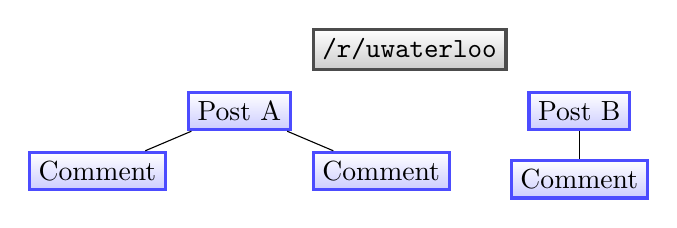
\begin{tikzpicture}[node distance=1em]
    \node (subreddit) [plain] {\texttt{/r/uwaterloo}};
    \node (post_a) [post, below left=of subreddit] {Post A};
    \node (post_b) [post, below right=of subreddit] {Post B};
    \node (comment_1) [post,below left=of post_a] {Comment};
    \node (comment_2) [post,below right=of post_a] {Comment};
    \node (comment_3) [post,below = of post_b] {Comment};

    \path (post_a) edge[-] (comment_1)
          (post_a) edge[-] (comment_2);
    \path (post_b) edge[-] (comment_3);

  \end{tikzpicture}
  \caption{Graph-like structure of the Reddit platform.}
  \label{fig:model:reddit}
\end{figure}

\subsection{Graph Model}
Two models are used for analysis. The first models how influential content or users are on a given subreddit as a connection between two graphs. A visualization of the structure can be found in Figure~\ref{fig:model:hypergraph}. Graph \(G_P\) is the graph that captures the inherent structural relationship between submissions/comments. Assumptions~\ref{assume:1} and~\ref{assume:2} imply that a given submission is influenced by its comments. More generally, any parent content is directly influenced by its children. These are visualized as the blue edges in Figure~\ref{fig:model:hypergraph}. This is augmented using edges that relate users to submissions/comments. The second model attempts to capture which users converse with each other. This graph, \(G_U\), can be thought of as being generated by the graph created above.

\begin{figure}
  \centering
  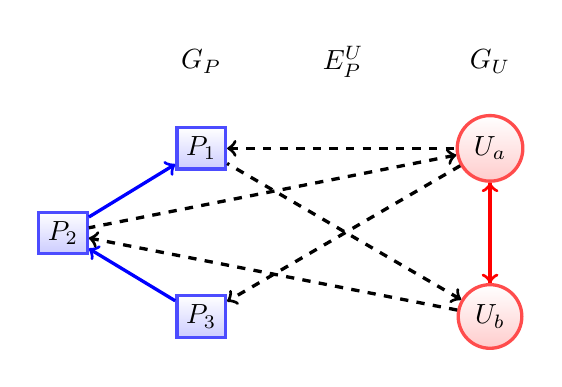
\begin{tikzpicture}[node distance=1em]
    \matrix[row sep=1em, column sep=3em] {
      & \node {$G_P$};& \node {$E_P^U$}; & \node {$G_U$};\\
      & \node (post_a) [post] {$P_1$}; & & \node (user_a) [user] {$U_a$};\\
      \node (comment_1) [post] {$P_2$}; & & & \\
      & \node (comment_2) [post] {$P_3$}; & &\node (user_b) [user] {$U_b$};\\
    };

    \path (post_a) edge[<-, blue, very thick] (comment_1)
          (comment_1) edge[<-, blue, very thick] (comment_2);

    \path (post_a) edge[<-, dashed, very thick] (user_a);
    \path (user_b) edge[<-, dashed, very thick] (post_a)
          (user_b) edge[->, dashed, very thick] (comment_1);
    \path (user_a) edge[<-, dashed, very thick] (comment_1)
          (user_a) edge[->, dashed, very thick] (comment_2);

    \path (user_a) edge[<-, red, very thick] (user_b)
          (user_a) edge[->, red, very thick] (user_b);
  \end{tikzpicture} 
  \caption{Graph structure showing the relationship between users and submissions/comments. \(G_P\) are those nodes and edges that are blue. \(G_U\) are those nodes and edges that are red. \(E_P^U\) is the set of edges denoted by broken lines.}
  \label{fig:model:hypergraph}
\end{figure}

\subsubsection{Graph Model for Centrality Analysis}
Denote the set of users by \(U\) and the set of submissions and comments by \(P.\) We first define the existence of the digraph \(G_P=(P,E_P)\) that denotes the relationship between submissions and comments. \(E_P\) is constructed in the manner described in Algorithm~\ref{alg:ep}.
\begin{algorithm}
  \ForAll{\(\mathtt{parent} \in P\)}{
    \For{\(\mathtt{child} \in P \cap ChildrenOf(P)\)}{
      \(E_P \gets E_P \cup \left\{ (\mathtt{parent}, \mathtt{child}) \right\} \)\;
    }
  }
  \caption{Constructing \(E_P.\)}
  \label{alg:ep}
\end{algorithm}
We give edges in \(E_P\) a universal weight of \(1.\) Weighting using upvotes was considered but was determined to yield results that were not desireable. For one, it was not clear that upvotes were a meaningful method of ranking influence. Further complexity arises when considering controversial content, which has a mix of upvotes and downvotes. A highly controversial topic may be highly influential, which contradicts the idea that upvotes correlate with influence. Possibly given knowledge of the number of voters this problem could be alleviated. However, since not all subreddits release data about how many users voted, it is simpler to reduce the complexity by eliminating any non-trivial weighting method. Observe that \(G_P\) is a forest where the submissions act as roots of the trees.

This structure is not interesting by itself and we need to extend it in order to facilitate analysis. The set of edges \(E_P^U\), that connects submissions/comments to users, is what brings the significant cross-post structure. \(E_P^U\) is generated in the manner described by Algorithm~\ref{alg:epu}. The rules are that: a comment author is influenced by the submission (root in \(G_P\)) and a comment author influences the comment. A more convoluted structure may be derived by instead having the comment author be influenced by the immediate parent comment. This structure was not investigated and could yield differing results. The argument for choosing the structure defined here is that authors may bring the whole context of the submission to a given comment, and not just the parent comment. The directed edge from the author to the submission allows us to model this sort of behaviour. That is, the user is influenced by all content on the submission page. This does ignore temporal effects, and so could yield incorrect results. On the other hand, the model not investigated is not as susceptible to temporal effects as it directly captures the temporal structure. However, it leaves out the ability to model any sort of larger contextual awareness the user may have.
\begin{algorithm}
  \ForAll{\(\mathtt{user} \in U\)}{
    \For{\(p \in P\) and \(\mathtt{user} = AuthorOf(p)\)}{
      \(\mathtt{root} \gets RootOf(p)\)\;
      \(E_P^U \gets E_P^U \cup \left\{ (p, \mathtt{user}), (\mathtt{user}, \mathtt{root}) \right\}\)\;
    }
  }
  \caption{Constructing \(E_P^U.\)}
  \label{alg:epu}
\end{algorithm}
The structure described above may be augmented with self-edges for all users and aperiodicity of the resulting graph can be guaranteed.
\begin{claim}
  Let the set of vertices be \(N = P \cup U.\) We also let \(E_N = E_P \cup E_P^U \cup \hat{E}\) be a set of edges, where \(\hat{E}\) is the set of directed self-edges for all users in \(U.\) Then \(G' = (N, E_N)\) is an aperiodic graph.
  \label{claim:g1:aperiodic}
\end{claim}
\begin{proof}
  Easy to see by the fact that cycles of any length may be constructed by including the users in the cycles. The simplest cycle may be constructed (see Figure~\ref{fig:model:hypergraph}) using a commenting user and the associated submission.
\end{proof}

\subsubsection{Graph Model for Cluster Analysis}
Submissions and comments are not directly significant for identifying subgroups within a community of users. The model used here is restricted to a weighted digraph \(G_U = (U, E_U, W_U).\) However, we desire a method of constructing relationships between users that capture ``interaction'' between users. Algorithm~\ref{alg:eu} defines one such construction. It captures the idea that a user Bob is influenced strongly by another user Jenn if Bob comments a lot on content Jenn submits. The algorithm adds an additional requirement: that the interactions are unique modulo the root submission. This additional restrition attempts to count the number of ``conversations'' taking place between users without the need for explicit start and stop points.
\begin{algorithm}
  \ForAll{\(p \in RootsOf(P)\)}{
    \(\mathtt{conversations} \gets \emptyset\)\;
    \For{\(p_2 \in ChildrenOf(p)\)}{
      \;
    }
  }
  \caption{Constructing \(E_U.\)}
  \label{alg:eu}
\end{algorithm}
{\red Complete explanation of the graph used for cluster analysis.}

\section{IMPLEMENTATION}
There are two methods of collecting Reddit submission and comment data. There is a live application programming interface (API) available for use, that provides live up-to-date data. The most natural API request available for downloading submissions is limited to the last 1000 submissions on a given subreddit. This substantially limits the amount of data available for collection; for some subreddits this constitutes only a few weeks of data. Other methods to getting this old data exist, but involve using the API in a convoluted manner. A user {\red find reddit user} addressed this problem and collated all data on Reddit for over ten years for the purpose of data analytics. The data can be found online, freely available for use, in an archived format~\cite{Software:RedditArchive}. Submissions and comments are stored in separate archives, organized by months or days. The data is stored in these files as compressed, line-delimited Javascript Objects (JSON).

The analysis focusses on data for the time frame starting at November 2017 and ending in February 2018. I developed a Python script that filters out unnecessary data from these archives and inserts the useful data into a Redis database, a fast in-memory key-value database~\cite{Software:Redis}. The software developed for this project and used for analysis is publicly available on Github~\cite{Software:Mine}.

\subsection{Centrality Analysis}
For measuring the influence of any given user or content, I propose using the Katz centrality measure. Centrality measures provide a measure of how ``central'' a node in a graph is. The simplest of measures simply counts the in-degree of a node. The Katz centrality measure is defined as,
\begin{definition}
  Let \(A\in \R^{n\times n}\) be an adjacency matrix for an aperiodic graph \(G.\) Let \(0 < \alpha < \rho(A)\). The Katz centrality measure for node \(i\) is defined as,
  \[
    c_i = \sum_{k=1}^\infty{ \sum_{j=1}^n {\alpha^k \left( A^k \right)_{j,i}} }.
  \]
\end{definition}
This measure counts the number of paths from all nodes in the graph to a given node \(i\), scoring paths of shorter length with a higher weight. The graph \(G'\) was shown in Claim~\cite{claim:g1:aperiodic} to be aperiodic and so we can use the Katz centrality measure on the induced adjacency matrix. Since \(G'\) is unweighted, we choose the natural weighting of \(1\) for all edges in the adjacency matrix. The implementation used is a custom script that employs an iterative technique that converges to the Katz centrality measure for all nodes~\cite{Notes:Network}.

\subsection{Cluster Analysis}
Spectral clustering is a family of techniques used for identifying disconnected components in a graph or, more generally, clusters of highly connected nodes using the graph Laplacian matrix. A survey of these techniques can be found in~\cite{Article:Survey}. I instead follow a variation of the simplest technique described in~\cite{Notes:Laplacian, Article:LaplacianTutorial}. We recall significant results used for spectral clustering now,
\begin{definition}
  Let \(A\in\R^{n \times n}\) and \(D\in\R^{n\times n}\) be the adjacency and out-degree matrix for the graph \(G_U.\) The graph Laplacian is defined as,
  \[
    L = D - A.
  \]
  The normalized graph Laplacian is defined as,
  \[
    L_{rw} = I - D^{-1}A.
  \]
\end{definition}
\begin{theorem}[Properties of the Graph Laplacian~\cite{Notes:Network}]
  The graph Laplacian and the normalized graph Laplacian enjoy the following properties,
  \begin{enumerate}[label=(\alph*)]
    \item{
      Say graph \(G_U\) has \(n\) nodes with \(k\) connected components. Then \[\rank L_{rw} = \rank L = n - k.\]
    }
    \item{
      The vector of all ones, \(\mathbf{1} \in \R^n\), is in \(\ker L_{rw} = \ker L.\) This vector evalutes the membership of all nodes to the graph.
    }
    \item{
      The eigenvalues \(\lambda_i\) of \(L\) and \(L_{rw}\) can be arranged in the following manner,
      \[
        0 = \Re\{\lambda_1\} \leq \Re\{\lambda_2\} \leq \cdots \leq \Re\{\lambda_n\}.
      \]
    }
  \end{enumerate}
\end{theorem}
The methodology to find a cluster within a graph is to bootstrap a clustering technique used in \(\R^m\), the \(k\)-means algorithm, by the eigenvectors of \(L_{rw}.\) This relies on the observation that the eigenvectors associated with eigenvalues at 0 are those that denote membership to a given connected component of the graph. Moreover, eigenvectors near zero can be thought of as measuring a partial membership to a cluster. As a result, we wish to find the eigenvectors of \(L_{rw}\) whose eigenvalues are near 0. This is not the best approach due to numerical instability of the eigenvalue algorithms used for sparse matrices. The choice to use \(L_{rw}\) alleviates the problems introduced by having a poor condition number, however we need to also employ a technique discussed by Frederix and Barel. They suggest instead looking at the matrix~\cite{Article:CholeskyLaplacian},
\[
  \hat{L}_{rw} = D^{-1}A.
\]
The matrix \(\hat{L}_{rw}\) has the same eigenvectors as \(L_{rw}\) while the eigenvalues shift. The eigenvalues instead move to be less than, or equal to, 1. This reformulation turns out to be much better suited to the numerical algorithms implemented to find eigenvalues of large sparse matrices.
%{Article:CholeskyLaplacian}.

\section{ANALYSIS}
One subreddit of particular interest to myself is the \texttt{/r/uwaterloo} subreddit. This community consists to date over 26 thousand subscribers. The subreddit is famous for a goose-related subculture that resulted in a man receiving a goose tattoo on an unsavoury location of his body~\cite{Website:GooseTattoo}.

%\addtolength{\textheight}{-12cm}   % This command serves to balance the column lengths
                                  % on the last page of the document manually. It shortens
                                  % the textheight of the last page by a suitable amount.
                                  % This command does not take effect until the next page
                                  % so it should come on the page before the last. Make
                                  % sure that you do not shorten the textheight too much.

%%%%%%%%%%%%%%%%%%%%%%%%%%%%%%%%%%%%%%%%%%%%%%%%%%%%%%%%%%%%%%%%%%%%%%%%%%%%%%%%



%%%%%%%%%%%%%%%%%%%%%%%%%%%%%%%%%%%%%%%%%%%%%%%%%%%%%%%%%%%%%%%%%%%%%%%%%%%%%%%%



%%%%%%%%%%%%%%%%%%%%%%%%%%%%%%%%%%%%%%%%%%%%%%%%%%%%%%%%%%%%%%%%%%%%%%%%%%%%%%%%
%\section*{APPENDIX}
%Appendixes should appear before the acknowledgment.

\section*{ACKNOWLEDGEMENT}
The author thanks Professor John Simpson for offering the special topics course on Networked and Distributed control, thereby providing the essential background for this analysis. The author also gives a special thanks to Jason Baumgartner for uploading archived Reddit API data to \cite{Software:RedditArchive}.

%%%%%%%%%%%%%%%%%%%%%%%%%%%%%%%%%%%%%%%%%%%%%%%%%%%%%%%%%%%%%%%%%%%%%%%%%%%%%%%%
\bibliography{IEEEabrv,root.bib}

\end{document}
